\documentclass[11pt]{article}
\usepackage[a4paper,landscape,margin=12mm]{geometry}
\usepackage{tikz}
\usetikzlibrary{arrows.meta}
\pagestyle{empty}
\setlength{\parindent}{0pt}
\begin{document}
\begin{center}
{\Large\bfseries Five-state extremal seed graphs}\par
\vspace{2mm}
All five rooted isomorphism classes attaining $H(G)=15$.
\par\vspace{3mm}
\begin{tabular}{@{}c@{\hspace{10mm}}c@{\hspace{10mm}}c@{}}
% Five-state extremal seed graph (a).
% Requires \usepackage{tikz} and \usetikzlibrary{arrows.meta}.
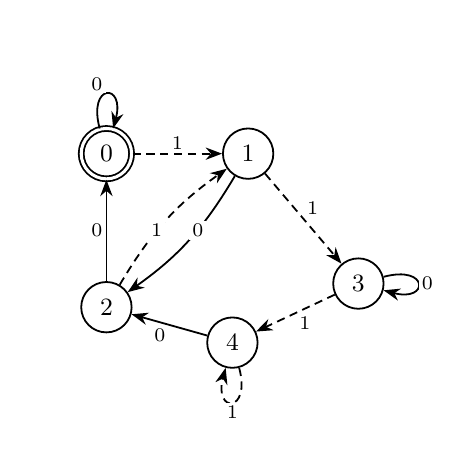
\begin{tikzpicture}[
  x=1cm,y=1cm,>=Stealth,
  f1m5 vertex/.style={circle,draw=black,line width=.65pt,minimum size=6.4mm,inner sep=0pt,font=\small},
  f1m5 root/.style={f1m5 vertex,double,double distance=1.1pt},
  f1m5 port zero/.style={->,draw=black,line width=.65pt},
  f1m5 port one/.style={->,draw=black,line width=.65pt,dash pattern=on 3pt off 2pt},
  f1m5 label/.style={font=\scriptsize,fill=white,inner sep=1.1pt}
]
\path[use as bounding box] (-2.60,-2.65) rectangle (2.60,2.65);
\node[f1m5 root] (q0) at (-1.60,1.05) {$ 0 $};
\node[f1m5 vertex] (q1) at (0.20,1.05) {$ 1 $};
\node[f1m5 vertex] (q2) at (-1.60,-0.90) {$ 2 $};
\node[f1m5 vertex] (q3) at (1.60,-0.60) {$ 3 $};
\node[f1m5 vertex] (q4) at (0.00,-1.35) {$ 4 $};
% edge 0 0 0
\draw[f1m5 port zero] (q0) edge[loop above,min distance=6mm] node[f1m5 label,above left] {$ 0 $} (q0);
% edge 0 1 1
\draw[f1m5 port one] (q0) edge[] node[f1m5 label,above] {$ 1 $} (q1);
% edge 1 0 2
\draw[f1m5 port zero] (q1) edge[bend left=12] node[f1m5 label,above right] {$ 0 $} (q2);
% edge 1 1 3
\draw[f1m5 port one] (q1) edge[] node[f1m5 label,above right] {$ 1 $} (q3);
% edge 2 0 0
\draw[f1m5 port zero] (q2) edge[] node[f1m5 label,left] {$ 0 $} (q0);
% edge 2 1 1
\draw[f1m5 port one] (q2) edge[bend left=12] node[f1m5 label,below left] {$ 1 $} (q1);
% edge 3 0 3
\draw[f1m5 port zero] (q3) edge[loop right,min distance=6mm] node[f1m5 label,right] {$ 0 $} (q3);
% edge 3 1 4
\draw[f1m5 port one] (q3) edge[] node[f1m5 label,below right] {$ 1 $} (q4);
% edge 4 0 2
\draw[f1m5 port zero] (q4) edge[] node[f1m5 label,below left] {$ 0 $} (q2);
% edge 4 1 4
\draw[f1m5 port one] (q4) edge[loop below,min distance=6mm] node[f1m5 label,below] {$ 1 $} (q4);
\end{tikzpicture}
&% Five-state extremal seed graph (b).
% Requires \usepackage{tikz} and \usetikzlibrary{arrows.meta}.
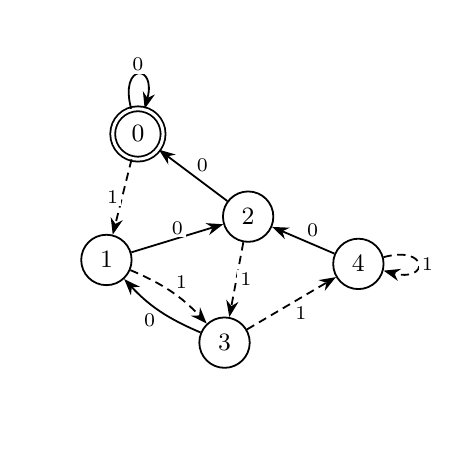
\begin{tikzpicture}[
  x=1cm,y=1cm,>=Stealth,
  f1m5 vertex/.style={circle,draw=black,line width=.65pt,minimum size=6.4mm,inner sep=0pt,font=\small},
  f1m5 root/.style={f1m5 vertex,double,double distance=1.1pt},
  f1m5 port zero/.style={->,draw=black,line width=.65pt},
  f1m5 port one/.style={->,draw=black,line width=.65pt,dash pattern=on 3pt off 2pt},
  f1m5 label/.style={font=\scriptsize,fill=white,inner sep=1.1pt}
]
\path[use as bounding box] (-2.60,-2.65) rectangle (2.60,2.65);
\node[f1m5 root] (q0) at (-1.20,1.30) {$ 0 $};
\node[f1m5 vertex] (q1) at (-1.60,-0.30) {$ 1 $};
\node[f1m5 vertex] (q2) at (0.20,0.25) {$ 2 $};
\node[f1m5 vertex] (q3) at (-0.10,-1.35) {$ 3 $};
\node[f1m5 vertex] (q4) at (1.60,-0.35) {$ 4 $};
% edge 0 0 0
\draw[f1m5 port zero] (q0) edge[loop above,min distance=6mm] node[f1m5 label,above] {$ 0 $} (q0);
% edge 0 1 1
\draw[f1m5 port one] (q0) edge[] node[f1m5 label,left] {$ 1 $} (q1);
% edge 1 0 2
\draw[f1m5 port zero] (q1) edge[] node[f1m5 label,above] {$ 0 $} (q2);
% edge 1 1 3
\draw[f1m5 port one] (q1) edge[bend left=12] node[f1m5 label,above right] {$ 1 $} (q3);
% edge 2 0 0
\draw[f1m5 port zero] (q2) edge[] node[f1m5 label,above right] {$ 0 $} (q0);
% edge 2 1 3
\draw[f1m5 port one] (q2) edge[] node[f1m5 label,right] {$ 1 $} (q3);
% edge 3 0 1
\draw[f1m5 port zero] (q3) edge[bend left=12] node[f1m5 label,below left] {$ 0 $} (q1);
% edge 3 1 4
\draw[f1m5 port one] (q3) edge[] node[f1m5 label,below right] {$ 1 $} (q4);
% edge 4 0 2
\draw[f1m5 port zero] (q4) edge[] node[f1m5 label,above right] {$ 0 $} (q2);
% edge 4 1 4
\draw[f1m5 port one] (q4) edge[loop right,min distance=6mm] node[f1m5 label,right] {$ 1 $} (q4);
\end{tikzpicture}
&% Five-state extremal seed graph (c).
% Requires \usepackage{tikz} and \usetikzlibrary{arrows.meta}.
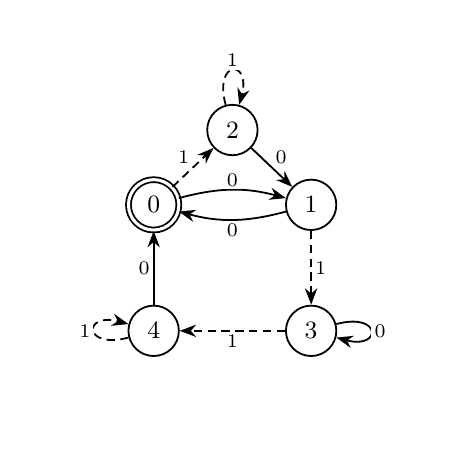
\begin{tikzpicture}[
  x=1cm,y=1cm,>=Stealth,
  f1m5 vertex/.style={circle,draw=black,line width=.65pt,minimum size=6.4mm,inner sep=0pt,font=\small},
  f1m5 root/.style={f1m5 vertex,double,double distance=1.1pt},
  f1m5 port zero/.style={->,draw=black,line width=.65pt},
  f1m5 port one/.style={->,draw=black,line width=.65pt,dash pattern=on 3pt off 2pt},
  f1m5 label/.style={font=\scriptsize,fill=white,inner sep=1.1pt}
]
\path[use as bounding box] (-2.60,-2.65) rectangle (2.60,2.65);
\node[f1m5 root] (q0) at (-1.00,0.40) {$ 0 $};
\node[f1m5 vertex] (q1) at (1.00,0.40) {$ 1 $};
\node[f1m5 vertex] (q2) at (0.00,1.35) {$ 2 $};
\node[f1m5 vertex] (q3) at (1.00,-1.20) {$ 3 $};
\node[f1m5 vertex] (q4) at (-1.00,-1.20) {$ 4 $};
% edge 0 0 1
\draw[f1m5 port zero] (q0) edge[bend left=15] node[f1m5 label,above] {$ 0 $} (q1);
% edge 0 1 2
\draw[f1m5 port one] (q0) edge[] node[f1m5 label,above left] {$ 1 $} (q2);
% edge 1 0 0
\draw[f1m5 port zero] (q1) edge[bend left=15] node[f1m5 label,below] {$ 0 $} (q0);
% edge 1 1 3
\draw[f1m5 port one] (q1) edge[] node[f1m5 label,right] {$ 1 $} (q3);
% edge 2 0 1
\draw[f1m5 port zero] (q2) edge[] node[f1m5 label,above right] {$ 0 $} (q1);
% edge 2 1 2
\draw[f1m5 port one] (q2) edge[loop above,min distance=6mm] node[f1m5 label,above] {$ 1 $} (q2);
% edge 3 0 3
\draw[f1m5 port zero] (q3) edge[loop right,min distance=6mm] node[f1m5 label,right] {$ 0 $} (q3);
% edge 3 1 4
\draw[f1m5 port one] (q3) edge[] node[f1m5 label,below] {$ 1 $} (q4);
% edge 4 0 0
\draw[f1m5 port zero] (q4) edge[] node[f1m5 label,left] {$ 0 $} (q0);
% edge 4 1 4
\draw[f1m5 port one] (q4) edge[loop left,min distance=6mm] node[f1m5 label,left] {$ 1 $} (q4);
\end{tikzpicture}
\\[-1mm]
(a)&(b)&(c)
\end{tabular}
\par\vspace{4mm}
\begin{tabular}{@{}c@{\hspace{10mm}}c@{}}
% Five-state extremal seed graph (d).
% Requires \usepackage{tikz} and \usetikzlibrary{arrows.meta}.
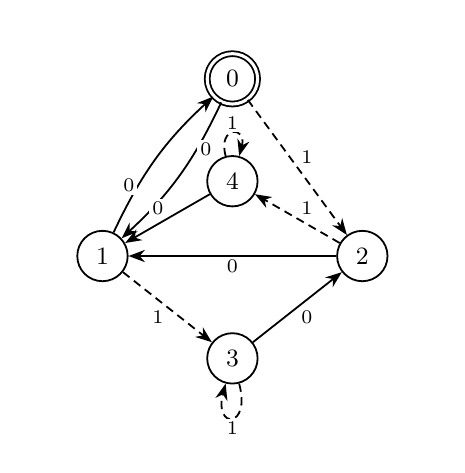
\begin{tikzpicture}[
  x=1cm,y=1cm,>=Stealth,
  f1m5 vertex/.style={circle,draw=black,line width=.65pt,minimum size=6.4mm,inner sep=0pt,font=\small},
  f1m5 root/.style={f1m5 vertex,double,double distance=1.1pt},
  f1m5 port zero/.style={->,draw=black,line width=.65pt},
  f1m5 port one/.style={->,draw=black,line width=.65pt,dash pattern=on 3pt off 2pt},
  f1m5 label/.style={font=\scriptsize,fill=white,inner sep=1.1pt}
]
\path[use as bounding box] (-2.60,-2.65) rectangle (2.60,2.65);
\node[f1m5 root] (q0) at (0.00,2.00) {$ 0 $};
\node[f1m5 vertex] (q1) at (-1.65,-0.25) {$ 1 $};
\node[f1m5 vertex] (q2) at (1.65,-0.25) {$ 2 $};
\node[f1m5 vertex] (q3) at (0.00,-1.55) {$ 3 $};
\node[f1m5 vertex] (q4) at (0.00,0.70) {$ 4 $};
% edge 0 0 1
\draw[f1m5 port zero] (q0) edge[bend left=11] node[f1m5 label,pos=.30,right] {$ 0 $} (q1);
% edge 0 1 2
\draw[f1m5 port one] (q0) edge[] node[f1m5 label,above right] {$ 1 $} (q2);
% edge 1 0 0
\draw[f1m5 port zero] (q1) edge[bend left=11] node[f1m5 label,pos=.30,left] {$ 0 $} (q0);
% edge 1 1 3
\draw[f1m5 port one] (q1) edge[] node[f1m5 label,below left] {$ 1 $} (q3);
% edge 2 0 1
\draw[f1m5 port zero] (q2) edge[] node[f1m5 label,below] {$ 0 $} (q1);
% edge 2 1 4
\draw[f1m5 port one] (q2) edge[] node[f1m5 label,above right] {$ 1 $} (q4);
% edge 3 0 2
\draw[f1m5 port zero] (q3) edge[] node[f1m5 label,below right] {$ 0 $} (q2);
% edge 3 1 3
\draw[f1m5 port one] (q3) edge[loop below,min distance=6mm] node[f1m5 label,below] {$ 1 $} (q3);
% edge 4 0 1
\draw[f1m5 port zero] (q4) edge[] node[f1m5 label,above left] {$ 0 $} (q1);
% edge 4 1 4
\draw[f1m5 port one] (q4) edge[loop above,min distance=4mm] node[f1m5 label,above] {$ 1 $} (q4);
\end{tikzpicture}
&% Five-state extremal seed graph (e).
% Requires \usepackage{tikz} and \usetikzlibrary{arrows.meta}.
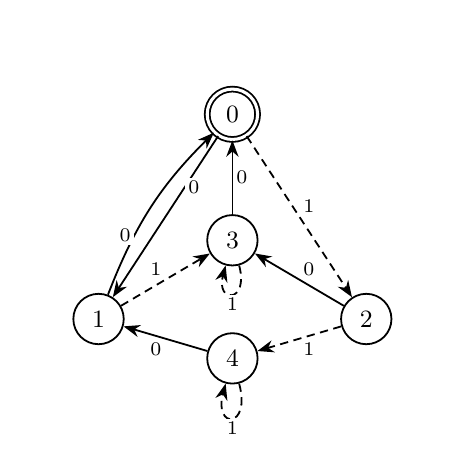
\begin{tikzpicture}[
  x=1cm,y=1cm,>=Stealth,
  f1m5 vertex/.style={circle,draw=black,line width=.65pt,minimum size=6.4mm,inner sep=0pt,font=\small},
  f1m5 root/.style={f1m5 vertex,double,double distance=1.1pt},
  f1m5 port zero/.style={->,draw=black,line width=.65pt},
  f1m5 port one/.style={->,draw=black,line width=.65pt,dash pattern=on 3pt off 2pt},
  f1m5 label/.style={font=\scriptsize,fill=white,inner sep=1.1pt}
]
\path[use as bounding box] (-2.60,-2.65) rectangle (2.60,2.65);
\node[f1m5 root] (q0) at (0.00,1.55) {$ 0 $};
\node[f1m5 vertex] (q1) at (-1.70,-1.05) {$ 1 $};
\node[f1m5 vertex] (q2) at (1.70,-1.05) {$ 2 $};
\node[f1m5 vertex] (q3) at (0.00,-0.05) {$ 3 $};
\node[f1m5 vertex] (q4) at (0.00,-1.55) {$ 4 $};
% edge 0 0 1
\draw[f1m5 port zero] (q0) edge[] node[f1m5 label,pos=.32,right] {$ 0 $} (q1);
% edge 0 1 2
\draw[f1m5 port one] (q0) edge[] node[f1m5 label,above right] {$ 1 $} (q2);
% edge 1 0 0
\draw[f1m5 port zero] (q1) edge[bend left=12] node[f1m5 label,pos=.32,left] {$ 0 $} (q0);
% edge 1 1 3
\draw[f1m5 port one] (q1) edge[] node[f1m5 label,above left] {$ 1 $} (q3);
% edge 2 0 3
\draw[f1m5 port zero] (q2) edge[] node[f1m5 label,above right] {$ 0 $} (q3);
% edge 2 1 4
\draw[f1m5 port one] (q2) edge[] node[f1m5 label,below right] {$ 1 $} (q4);
% edge 3 0 0
\draw[f1m5 port zero] (q3) edge[] node[f1m5 label,right] {$ 0 $} (q0);
% edge 3 1 3
\draw[f1m5 port one] (q3) edge[loop below,min distance=5mm] node[f1m5 label,below] {$ 1 $} (q3);
% edge 4 0 1
\draw[f1m5 port zero] (q4) edge[] node[f1m5 label,below left] {$ 0 $} (q1);
% edge 4 1 4
\draw[f1m5 port one] (q4) edge[loop below,min distance=6mm] node[f1m5 label,below] {$ 1 $} (q4);
\end{tikzpicture}
\\[-1mm]
(d)&(e)
\end{tabular}
\par\vspace{4mm}
\begin{minipage}{20cm}
\centering\small
The root $0$ is marked by a double circle. Solid arrows denote port $\tau_0$;
dashed arrows denote port $\tau_1$. Edge labels give the port number.
Each drawing represents one seed graph, with its static masks varying over all
vertices.
\end{minipage}
\end{center}
\end{document}
